% Options for packages loaded elsewhere
\PassOptionsToPackage{unicode}{hyperref}
\PassOptionsToPackage{hyphens}{url}

\documentclass[12pt]{article}
\usepackage[margin=1in]{geometry} 
\usepackage{amsmath,amsthm,amssymb}
\usepackage{minted}
\usepackage{graphicx}   
\usepackage{tocloft}
\usepackage{hyperref}
\usepackage{array}
\usepackage{longtable}
\setlength{\parindent}{0pt}

\newcommand{\N}{\mathbb{N}}
\newcommand{\Z}{\mathbb{Z}}

\usepackage{booktabs}
\usepackage{float}
\usepackage{caption}
\usepackage{subcaption}
\usepackage{placeins}
\usepackage{lmodern}
\usepackage{xcolor}
\definecolor{darkgreen}{rgb}{0, 0.5, 0}
\definecolor{Valentia}{RGB}{233,78,82}
\definecolor{Titleblue}{RGB}{114, 146, 162}
\usepackage{mdframed}
\usepackage{multirow}
\usepackage{multicol}
\usepackage{scrextend}
\usepackage{tikz}
\usepackage{subcaption}
\usepackage[absolute]{textpos}
\usepackage{colortbl}
\usepackage{geometry}
\usepackage{listings}
\usepackage{verbatim}

\lstset{
  language=R,
  backgroundcolor=\color{white},   % Couleur de fond
  basicstyle=\ttfamily\small,      % Style de base du texte
  breaklines=true,                 % Saut de ligne automatique
  showstringspaces=false,          % Ne pas afficher les espaces dans les chaînes
  keywordstyle=\color{blue},       % Couleur des mots-clés
  commentstyle=\color{darkgreen},  % Couleur des commentaires
  stringstyle=\color{red},         % Couleur des chaînes
}

\pagestyle{plain}

 
\setminted{
  breaklines=true,      % Activer les retours à la ligne automatiques
  breakanywhere=true,   % Permet de casser les lignes n'importe où
}
\pagestyle{plain} % style simple : juste le numéro de page en bas


\begin{document}



\begin{titlepage}
    \centering
    
    \vspace{1cm}
    {\Huge {Apprentissage Statistique}}\\[1.5cm]
    
    \vspace{1cm}
    {\Huge \textbf{TP : SVM}}\\[2cm]
    
    {\large
    \textbf{Kaoutar SARIH}\\ \textbf{Doha EL QEMMAH}\\[2cm]}
    
    {\large Montpellier, le 3 octobre 2025}
    
    \vfill
    
    % Logo en bas
    
\includegraphics[width=0.5\textwidth]{images/logo.ssd.png}\\[0.5cm]
    
\end{titlepage}

\newpage

\tableofcontents 
\newpage  
\section*{Objectif du TP}
Ce TP a pour objectif de mettre en œuvre les Support Vector Machines (SVM) sur des jeux de données simulées (gaussiennes, Iris) et réelles (visages LFW).
Les points étudiés sont :
\begin{itemize}
  \item l’effet du noyau (linéaire, polynomial),
  \item l’influence du paramètre de régularisation $C$ et du paramètre $\gamma$,
  \item l’impact des données déséquilibrées et des variables de nuisance,
  \item l’amélioration possible via la réduction de dimension par PCA.
\end{itemize}


\subsection*{Jeu de données simulé : deux gaussiennes}

Nous commençons par générer un jeu de données simple composé de deux 
nuages gaussiens bidimensionnels. La figure ci-dessous illustre la 
distribution : chaque nuage correspond à une classe différente et 
est représenté par une couleur contrastée. 
On observe ainsi que l’ensemble est formé de deux sous-nuages 
distincts, issus de vecteurs gaussiens générés aléatoirement.

\begin{figure}[h!]
  \centering
  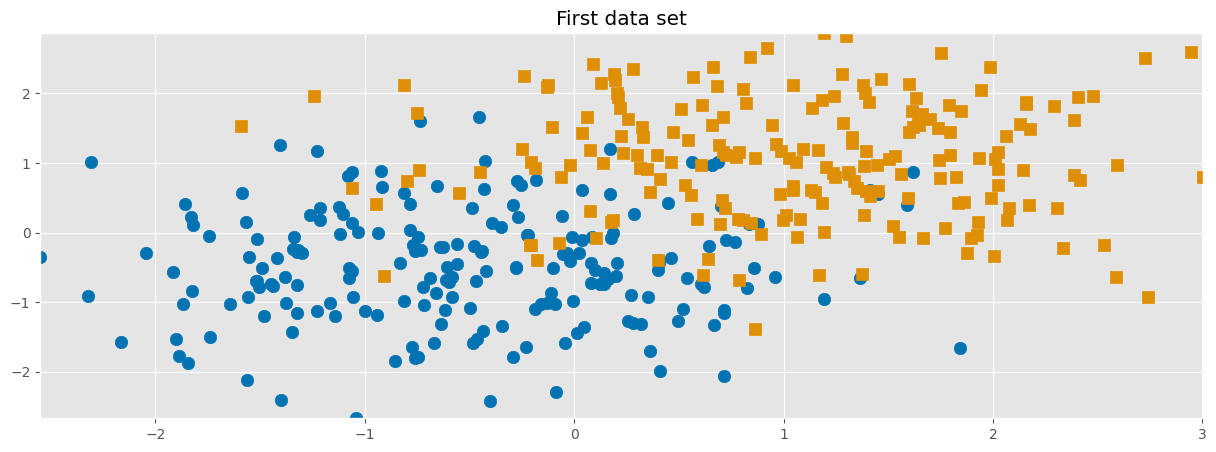
\includegraphics[width=0.6\textwidth]{images/gauss1.png}
  \caption{Premier jeu de données simulé : deux gaussiennes distinctes.}
\end{figure}
Nous discernons bien une séparation entre la majorité des points de 
chaque distribution gaussienne. Cependant, le choix d’un noyau linéaire 
implique qu’il reste des observations mal classées de part et d’autre 
de la frontière. 

\begin{figure}[h!]
  \centering
  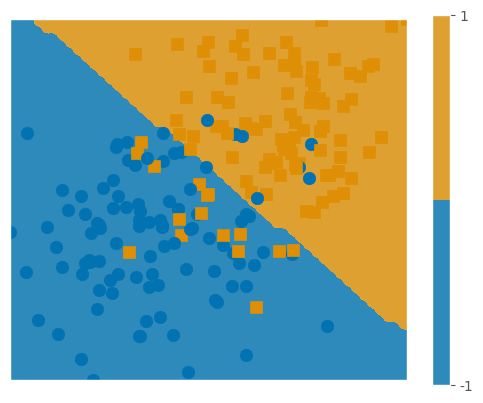
\includegraphics[width=0.25\textwidth]{images/gauus2.png}
  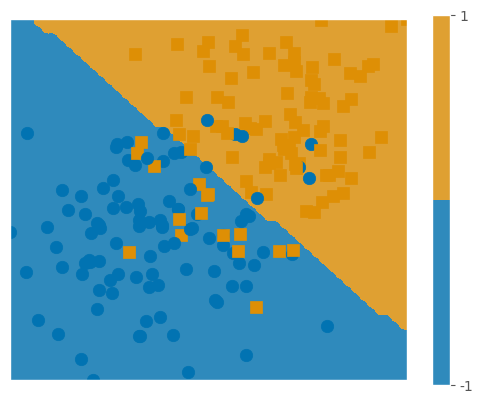
\includegraphics[width=0.25\textwidth]{images/gauss3.png}
  \caption{Frontière de décision d’un SVM à noyau linéaire sur les données gaussiennes.}
\end{figure}

Il apparaît que plusieurs valeurs du paramètre $C$ donnent un score 
d’environ $0.875$, ce qui semble correspondre à une valeur optimale. 
Néanmoins, le graphe obtenu n’est pas particulièrement plus convaincant 
que le précédent, ce qui suggère que le jeu de données choisi n’est pas 
idéal pour mettre en évidence les différences de performance entre 
paramètres et noyaux. Un jeu de données plus complexe permettrait sans 
doute une meilleure illustration.







\section{Question 1 et 2 : Iris avec noyau linéaire et polynomial}
Les étapes suivantes seront réalisées :
\begin{itemize}
  \item Normalisation des données et sélection des deux classes.
  \item Découpage en apprentissage/test.
  \item Recherche du meilleur $C$ avec GridSearchCV.
  \item Présenter les scores obtenus (train/test).
\end{itemize}

\subsection{Chargement et normalisation des données}

Nous utilisons le jeu de données \texttt{Iris} disponible dans la bibliothèque \texttt{scikit-learn}. 
Afin de simplifier le problème, nous nous limitons aux deux classes, 
et nous ne considérons que les deux premières caractéristiques (longueur et largeur du sépale).
\newline
L'étape de normalisation est indispensable en SVM et une variable ayant une échelle beaucoup plus grande que les autres aurait une influence disproportionnée sur la frontière de décision. Nous présentons ci-dessous un extrait des jeux de données 
d’apprentissage et de test utilisés pour l’entraînement du SVM. 

\begin{figure}[h!]
  \centering
  \begin{minipage}{0.48\textwidth}
    \centering
    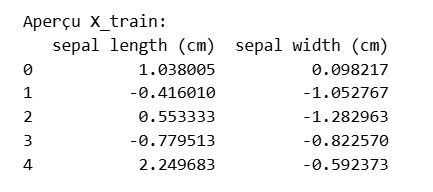
\includegraphics[width=\textwidth]{images/vis_train.jpg}
    \caption{Aperçu du jeu de train $X_{\text{train}}$.}
  \end{minipage}\hfill
  \begin{minipage}{0.48\textwidth}
    \centering
    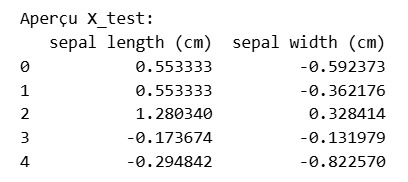
\includegraphics[width=\textwidth]{images/vis_xtest.jpg}
    \caption{Aperçu du jeu de test $X_{\text{test}}$.}
  \end{minipage}
\end{figure}


\subsection{Classification avec noyau linéaire}

Les données sont séparées aléatoirement en deux sous-ensembles : un ensemble d'apprentissage 
(\texttt{train}) et un ensemble de test (\texttt{test}). Nous entraînons ensuite un SVM avec noyau linéaire, 
en optimisant le paramètre de régularisation $C$ à l’aide d’une validation croisée.

Le meilleur paramètre trouvé est : 
\[
C = \texttt{0.8407}, \quad \text{noyau = linéaire}
\]

Les scores de généralisation obtenus sont :
\[
\text{Train} = 0.747 \quad\quad \text{Test} = 0.680
\]

Il est logique que le score obtenu sur l’ensemble d’apprentissage soit plus élevé que celui mesuré sur l’ensemble de test. Cela traduit le fait que le modèle s’adapte davantage aux données d’entraînement, tout en conservant une capacité correcte de généralisation. Avec le noyau linéaire et un paramètre $C$ optimal, la précision atteint environ 70\%.

\begin{figure}[h!]
  \centering
  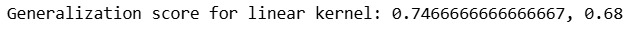
\includegraphics[width=0.85\textwidth]{images/lineaire_noyau.jpg}
\end{figure}

\subsection{Classification avec noyau polynomial}
 Passons maintenant au noyau polynomial :\\
Pour le noyau polynomial, l’optimisation a sélectionné le degré 1 comme valeur optimale, ce qui conduit à un modèle identique au cas linéaire. 
 \begin{figure}[h!]
  \centering
  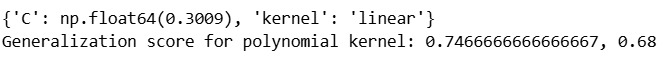
\includegraphics[width=0.85\textwidth]{images/poly_noyau_deg1.jpg}
\end{figure}

Le degré 1 ayant été sélectionné initialement (cas linéaire), nous avons volontairement exclu cette valeur et limité la recherche aux degrés 2 et 3 pour observer les performances du noyau polynomial dans un cadre non linéaire.
 \begin{figure}[h!]
  \centering
  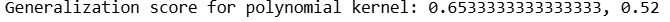
\includegraphics[width=0.85\textwidth]{images/poly_noyau_deg_2.jpg}
\end{figure}

 \begin{figure}[h!]
  \centering
  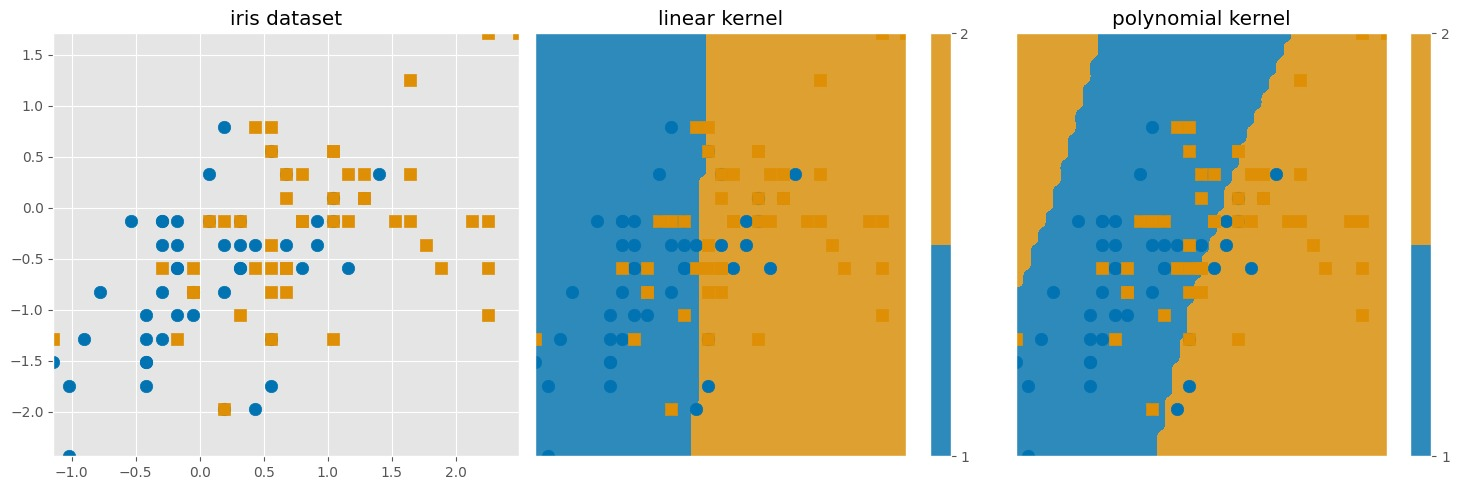
\includegraphics[width=0.75\textwidth]{images/lin_vs_poly.jpg}
\end{figure}

La représentation graphique montre que le noyau linéaire fournit une séparation simple et robuste, mais imparfaite en raison du chevauchement naturel des classes.
Le noyau polynomial introduit une frontière plus flexible, qui peut mieux séparer certaines observations mais au prix d’une complexité accrue et d’un risque de surapprentissage.
Ce comportement correspond exactement à ce qui est vu dans le cours : le choix du noyau doit refléter la nature de la distribution des données, en recherchant un compromis entre biais (modèle trop simple) et variance (modèle trop complexe).


\section{Question 3 : SVM Gui}
Nous avons suivi les indications du site 
\href{https://scikit-learn.org/1.2/auto_examples/applications/svm_gui.html}{scikit-learn svm\_gui} 
qui fournit le code source disponible dans \texttt{python\_script/svm\_gui.py}. 
Ce script est lancé en console.

Dans cette expérience, nous générons un jeu de données déséquilibré constitué 
de 20 points de la classe 1 (représentés en noir) et 4 points de la classe 2 
(représentés en blanc). L’objectif est d’ajuster une frontière de séparation en testant différents noyaux et paramètres.

Nous explorons le noyau linéaire avec les paramètres :
\begin{itemize}
    \item de régularisation $C$, qui détermine l’influence des erreurs de classification .
    \item $\gamma$, qui contrôle la distance d’influence d’un point donné .
\end{itemize}

Dans notre étude, nous avons principalement modifié le paramètre $C$ afin 
d’observer son impact sur la frontière de décision et la précision du modèle.

\begin{figure}[H]
    \centering
    \begin{subfigure}{0.32\textwidth}
        \centering
        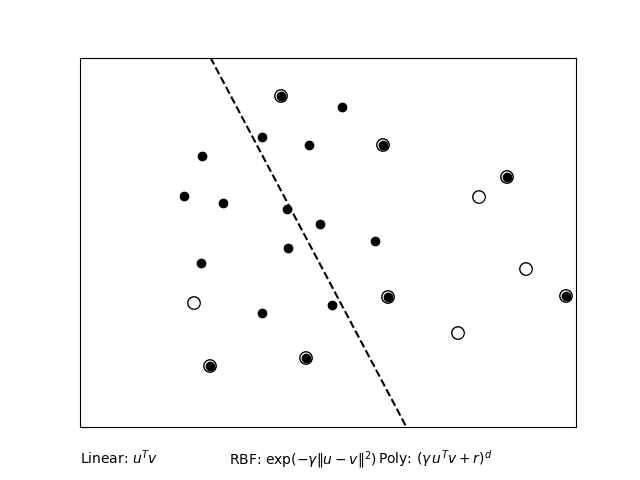
\includegraphics[width=\linewidth]{images/linC=0.01.png}
        \caption{Noyau linéaire $C=0.01$}
    \end{subfigure}
    \begin{subfigure}{0.32\textwidth}
        \centering
        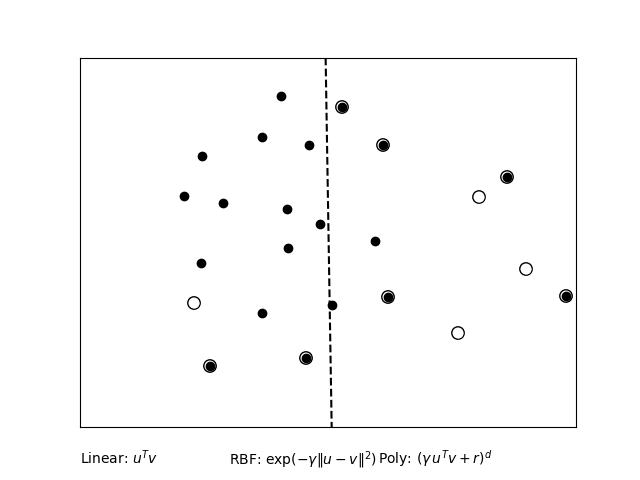
\includegraphics[width=\linewidth]{images/linC=1.png}
        \caption{Noyau linéaire $C=1$}
    \end{subfigure}
    \begin{subfigure}{0.32\textwidth}
        \centering
        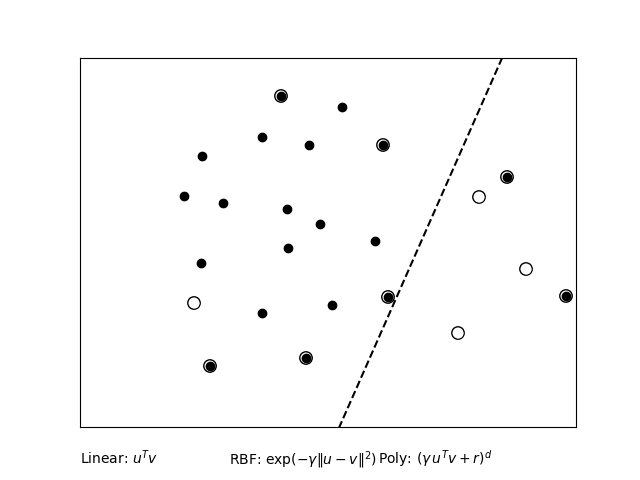
\includegraphics[width=\linewidth]{images/linC=7.png}
        \caption{Noyau linéaire $C=7$}
    \end{subfigure}
    \caption{Influence du paramètre de régularisation $C$ sur la frontière de décision (noyau linéaire).}
\end{figure}

\noindent
\textbf{Interprétation.}  
En observant les trois figures, on constate que la valeur de $C$ influence directement 
la position et l’inclinaison de la frontière de séparation. 

\begin{itemize}
    \item Pour $C=0.01$, la frontière est très approximative : elle ne cherche pas à bien séparer tous les points et tolère davantage d’erreurs de classification.
    \item Pour $C=1$, la séparation devient plus équilibrée. La frontière s’ajuste mieux à la répartition des données.
    \item Pour $C=7$, la frontière est beaucoup plus contrainte par les données. Le modèle cherche à corriger davantage de points mal classés.
\end{itemize}

En résumé, plus $C$ est petit, plus le modèle tolère les erreurs individuelles; à l’inverse, plus $C$ est grand, plus le modèle essaie de classer correctement chaque point.









\section{Classification des visages :}
\subsection{Question 4: }
\subsection*{Classification de visages avec noyau linéaire}

Nous utilisons la base de données LFW (Labeled Faces in the Wild) en restreignant 
le problème à deux individus : \textit{Tony Blair} et \textit{Colin Powell}. 

Les données sont centrées et réduites puis divisées en deux ensembles de taille égale : apprentissage 
(50\%) et test (50\%). Un SVM à noyau linéaire est entraîné en testant différents 
paramètres de régularisation $C$ sur une échelle logarithmique entre $10^{-5}$ et $10^{5}$.

\begin{figure}[h!]
  \centering
  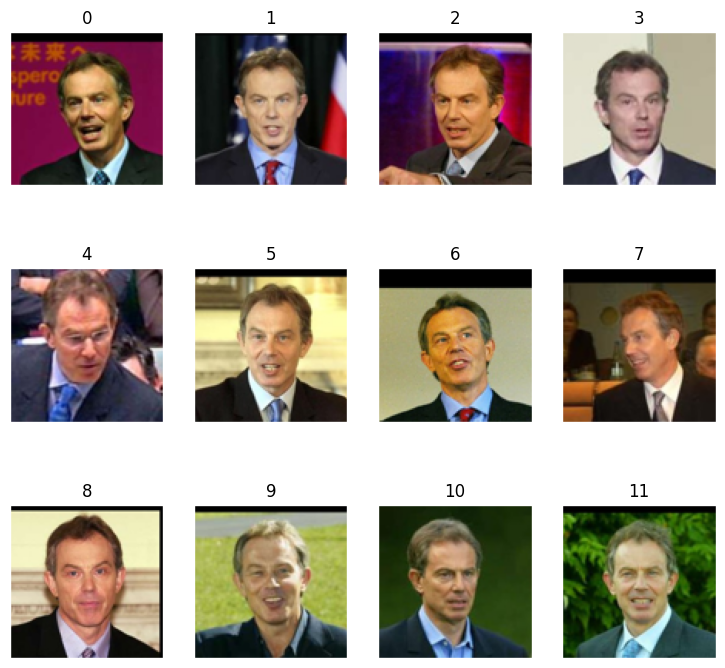
\includegraphics[width=0.8\textwidth]{images/faces1.png}
  \caption{Exemples d’images extraites du dataset LFW (Tony Blair).}
\end{figure}
\newpage
Le graphique ci-dessous montre l’évolution des scores et de l’erreur de test 
en fonction de  $C$:

\begin{figure}[h!]
  \centering
  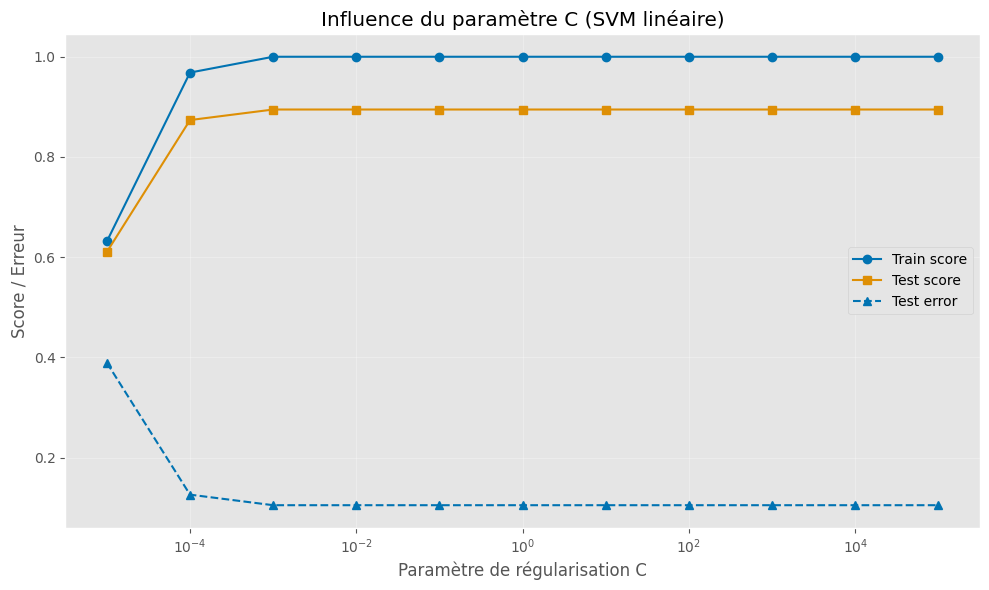
\includegraphics[width=0.8\textwidth]{images/Q4.png}
  \caption{Influence du paramètre de régularisation $C$.}
\end{figure}




Le meilleur paramètre obtenu est $C=0.001$. Avec ce choix, le modèle atteint 
une précision parfaite sur l’ensemble d’apprentissage (100\%), et une précision de à peu près 91\% sur l’ensemble de test. L’écart entre apprentissage et test montre un léger sur-apprentissage, mais les performances restent excellentes, nettement supérieures au niveau de hasard (62\%). \\




En plus de l’évaluation quantitative, nous avons analysé les résultats de la 
classification sur l’ensemble de test. La figure suivante illustre quelques prédictions réalisées par le modèle, avec comparaison entre l’étiquette prédite et l’étiquette réelle voir figure~\ref{fig:figure8}.\\

\begin{figure}[h!]
  \centering
  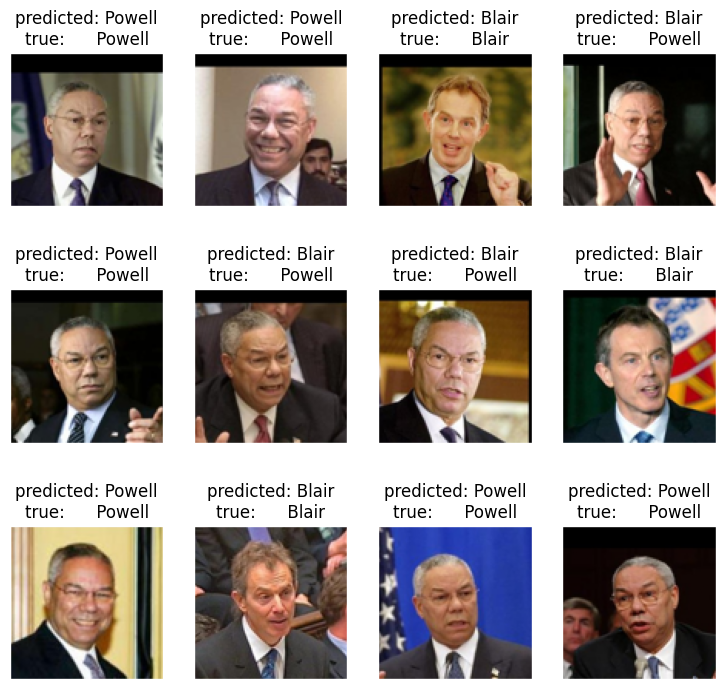
\includegraphics[width=0.7\textwidth]{images/prediction.png}
  \caption{nom prédit vs nom réel}
  \label{fig:figure8}
\end{figure}

Nous observons que la plupart des visages sont correctement classés, avec néanmoins quelques erreurs (3 mal prédits vs 9 correctement prédits).\\

Nous avons également visualisé la carte des coefficients du SVM linéaire entraîné avec le meilleur paramètre $C$ voir figure~\ref{fig:figure9}.

\begin{figure}[h!]
  \centering
  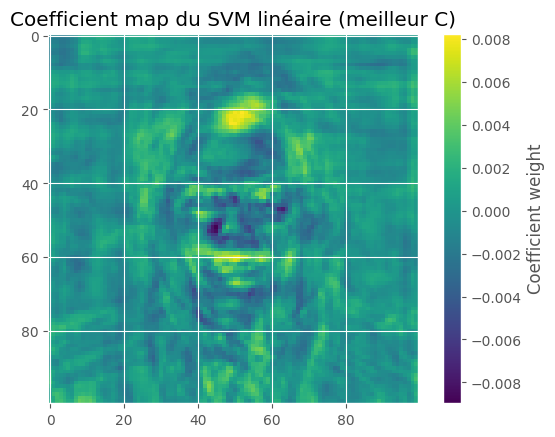
\includegraphics[width=0.6\textwidth]{images/C.png}
  \caption{Carte des coefficients du SVM linéaire.}
  \label{fig:figure9}
\end{figure}

Les zones les plus intenses dans la figure correspondent aux parties de l’image ayant le plus d’influence dans la décision. Cette représentation met en évidence que les zones centrales du visage (yeux, nez, bouche) 
contribuent le plus à la classification.
\newpage
\subsection{Question 5 : }
Pour évaluer la robustesse du modèle, nous avons ajouté 300 variables de 
nuisance générées aléatoirement (bruit gaussien) aux caractéristiques originales. 
Le SVM linéaire est ensuite ré-entraîné et évalué.

\begin{itemize}
  \item Sans variables de nuisance : 
  \textit{Score entraînement} = 1.0, \textit{Score test} = 0.879
  \item Avec variables de nuisance : 
  \textit{Score entraînement} = 1.0, \textit{Score test} = 0.584
\end{itemize}

Les résultats montrent que l’ajout de bruit n’affecte pas l’entraînement 
(le modèle parvient toujours à séparer les données d’apprentissage), 
mais entraîne une chute importante de la performance en test. 

Ce phénomène s’explique par le surapprentissage : 
le modèle utilise les variables parasites pour améliorer artificiellement 
son score d’entraînement, mais ces dimensions ne contiennent aucune information 
utile pour la classification, ce qui dégrade fortement sa capacité de généralisation.

\subsection{Question 6 : Amélioration par réduction de dimension (PCA)}

Afin de limiter l’effet des variables de nuisance ajoutées dans la 
question précédente, nous appliquons une réduction de dimension 
par Analyse en Composantes Principales (PCA) en utilisant 
\texttt{svd\_solver='randomized'}.

Avec $n\_components = 10$, les résultats obtenus sont :
\[
\text{Score train} = 0.60, \quad \text{Score test} = 0.64
\]

Comparé au cas précédent (sans PCA), où le score de test tombait à 
0.58 malgré un score d’entraînement parfait, la PCA améliore la 
capacité de généralisation du modèle. 

La réduction de dimension agit comme un filtre qui supprime le bruit 
et empêche le surapprentissage. Toutefois, un choix trop faible du 
nombre de composantes peut entraîner une perte d’information 
et donc un score global plus bas.\\
Nous avons toutefois rencontré un problème : le temps d’exécution de la PCA devient très important lorsque le nombre n augmente. Néanmoins, cela n’empêche pas de confirmer que la PCA joue bien son rôle de compromis entre réduction du bruit et conservation de l’information utile.

\subsection{Question 7 : Biais dans le prétraitement des données}

Dans notre pipeline initial dans le dataset d'images, nous avons normalisé les données (en centrant et réduisant chaque variable) avant la séparation 
entre apprentissage (train) et test. Ce choix introduit un biais, car 
les statistiques (moyenne et écart-type) sont calculées sur 
l’ensemble complet, incluant des informations provenant du jeu 
de test.
Ce phénomène correspond à une \textit{fuite d’information} : le modèle bénéficie indirectement 
d’informations sur le test, ce qui contredit la démarche que nous devons poursuir pour une réussite de prédiction et une dévaluation de ses 
performances.
La bonne pratique consiste à ajuster la normalisation uniquement 
sur l’ensemble train, puis à appliquer cette transformation au jeu de test.
\newpage
\appendix
\section*{Annexe}
Le code complet utilisé pour les expériences est disponible à l’adresse suivante : \\
\href{https://github.com/ksarih/TP_SVM}{https://github.com/ksarih/TP\_SVM}.
\end{document}
